\documentclass{beamer}

\usepackage{amsmath,amssymb}
\usepackage{tikz}
\usepackage{graphicx}
\usepackage{multicol}
\usepackage[per-mode=fraction]{siunitx}

\usetheme{Boadilla}
\usecolortheme{orchid}

\usetikzlibrary{calc}

\tikzset{>=stealth}

\usepackage{scalerel}

\newcommand*{\paral}{\stretchrel*{\parallel}{\perp}}


\title{PHYS2350: Forces}
\author{Dr. Wolf}
\date{Fall 2024}

\begin{document}

\begin{frame}
  \titlepage
\end{frame}

\begin{frame}
  {Quick Review:}
  \begin{block}{What is a force?}
    \begin{itemize}
      \item A push or a pull (it is a \textit{vector})
      \item An \textit{interaction} between \textit{two things}
    \end{itemize}
    Force notation:
    \[
      \vec{F}^{(\text{type})}_{A,B}
    \]
    Only these forces make up the \textit{net force} used in Newton's 2\textsuperscript{nd} Law
  \end{block}
  Common ``forces'' that will never appear on a free-body diagram
  \begin{columns}
    \begin{column}{0.4\textwidth}
      \begin{itemize}
        \item \textcolor{red}{Centripetal Force}: $ma_{\perp}$
        \item \textcolor{red}{Tangential Force}: $ma_{\paral}$
        \item \textcolor{blue}{Centrifugal Force}
        \item \textcolor{blue}{Tidal Force}
        \item \textcolor{blue}{Coriolis Force}
      \end{itemize}
    \end{column}
    \begin{column}{0.55\textwidth}
      \begin{center}
        \begin{exampleblock}{}
            All of these are either ways of characterizing the \textcolor{red}{net force} or
            forces that are a result of being in a \textcolor{blue}{non-inertial/accelerating
              reference frame}.
        \end{exampleblock}
      \end{center}
    \end{column}
  \end{columns}
\end{frame}

\begin{frame}
  {Part \textrm{I}. Constant speed}
  \begin{block}
    {Newton's 2\textsuperscript{nd} law}
    \[
      \vec{F}_{\text{net},\text{system}} = m_{\text{system}} \vec{a}_{\text{system}}
    \]
    If we have constant speed, and 1D motion, what is the acceleration?
  \end{block}
  \begin{columns}
    \begin{column}
      {0.5\textwidth}
      System A
      \begin{center}
        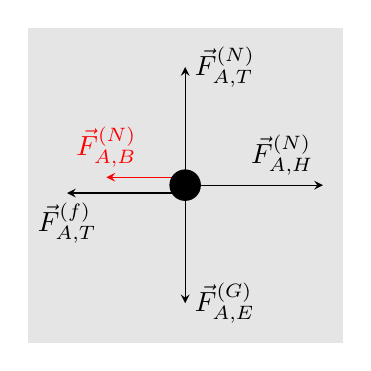
\begin{tikzpicture}
          \def\shift{0.1};
          \fill[black!10!white] (-2,-2) rectangle (2,2);
          \coordinate (O) at (0,0);
          \begin{scope}[->]
            \draw (O) -- +(0,-1.5) node [right]{$\vec{F}^{(G)}_{A,E}$};
            \draw (O) -- +(0,1.5) node [right]{$\vec{F}^{(N)}_{A,T}$};
            \draw (O) -- +(1.75,0) node [above left]{$\vec{F}^{(N)}_{A,H}$};
            \draw[red] ($(O) +(0,\shift)$) -- +(-1,0) node [above]{$\vec{F}^{(N)}_{A,B}$};
            \draw ($(O) +(0,-\shift)$) -- +(-1.5,0) node [below]{$\vec{F}^{(f)}_{A,T}$};
          \end{scope}
          \fill (O) circle (0.2);
        \end{tikzpicture}
      \end{center}
    \end{column}
    \begin{column}
      {0.5\textwidth}
      System B
      \begin{center}
        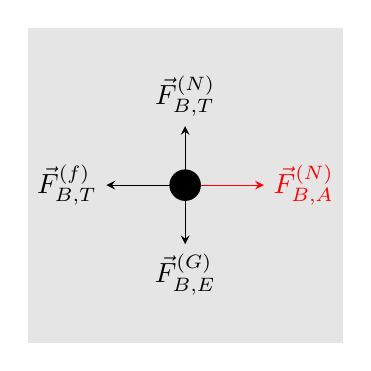
\begin{tikzpicture}
          \fill[black!10!white] (-2,-2) rectangle (2,2);
          \coordinate (O) at (0,0);
          \begin{scope}[->]
            \draw (O) -- +(0,-0.75) node [below]{$\vec{F}^{(G)}_{B,E}$};
            \draw (O) -- +(0,0.75) node [above]{$\vec{F}^{(N)}_{B,T}$};
            \draw (O) -- +(-1,0) node [left]{$\vec{F}^{(f)}_{B,T}$};
            \draw[red] (O) -- +(1,0) node [right]{$\vec{F}^{(N)}_{B,A}$};
          \end{scope}
          \fill (O) circle (0.2);
        \end{tikzpicture}
      \end{center}
    \end{column}
  \end{columns}
\end{frame}

\begin{frame}
  {Part \textrm{I}. Constant speed}
  \begin{columns}
    \begin{column}
      {0.5\textwidth}
      System A
      \begin{center}
        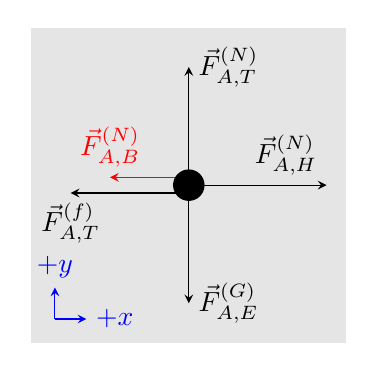
\begin{tikzpicture}
          \def\shift{0.1};
          \fill[black!10!white] (-2,-2) rectangle (2,2);
          \coordinate (O) at (0,0);
          \begin{scope}[->]
            \draw (O) -- +(0,-1.5) node [right]{$\vec{F}^{(G)}_{A,E}$};
            \draw (O) -- +(0,1.5) node [right]{$\vec{F}^{(N)}_{A,T}$};
            \draw (O) -- +(1.75,0) node [above left]{$\vec{F}^{(N)}_{A,H}$};
            \draw[red] ($(O) +(0,\shift)$) -- +(-1,0) node [above]{$\vec{F}^{(N)}_{A,B}$};
            \draw ($(O) +(0,-\shift)$) -- +(-1.5,0) node [below]{$\vec{F}^{(f)}_{A,T}$};
            \draw[blue] (-1.7,-1.7) -- +(0,0.4) node [above]{$+y$};
            \draw[blue] (-1.7,-1.7) -- +(0.4,0) node [right]{$+x$};
          \end{scope}
          \fill (O) circle (0.2);
        \end{tikzpicture}
      \end{center}
      Break into components\dotfill
      \begin{align*}
        F^{(N)}_{A,H} - F^{(N)}_{A,B} - F^{(f)}_{A,T} &= 0 \\
        F^{(N)}_{A,T} - F^{(G)}_{A,E} &= 0
      \end{align*}
    \end{column}
    \begin{column}
      {0.5\textwidth}
      System B
      \begin{center}
        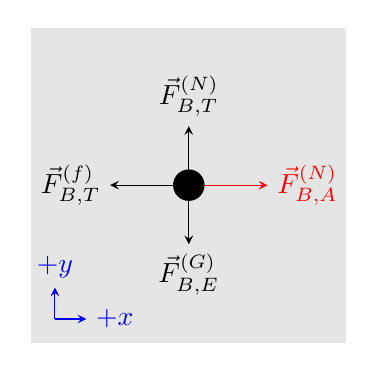
\begin{tikzpicture}
          \fill[black!10!white] (-2,-2) rectangle (2,2);
          \coordinate (O) at (0,0);
          \begin{scope}[->]
            \draw (O) -- +(0,-0.75) node [below]{$\vec{F}^{(G)}_{B,E}$};
            \draw (O) -- +(0,0.75) node [above]{$\vec{F}^{(N)}_{B,T}$};
            \draw (O) -- +(-1,0) node [left]{$\vec{F}^{(f)}_{B,T}$};
            \draw[red] (O) -- +(1,0) node [right]{$\vec{F}^{(N)}_{B,A}$};
            \draw[blue] (-1.7,-1.7) -- +(0,0.4) node [above]{$+y$};
            \draw[blue] (-1.7,-1.7) -- +(0.4,0) node [right]{$+x$};
          \end{scope}
          \fill (O) circle (0.2);
        \end{tikzpicture}
      \end{center}
      Considering magnitudes only
      \begin{align*}
        F^{(N)}_{B,A} - F^{(f)}_{B,T} &= 0 \\
        F^{(N)}_{B,T} - F^{(G)}_{B,E} &= 0
      \end{align*}
    \end{column}
  \end{columns}
\end{frame}

\begin{frame}
  {Part \textrm{I}. Vertical forces, calculating weight}
  For the vertical forces, we have:
  \[
    F^{(N)}_{A,T} = F^{(G)}_{A,E} \qquad F^{(N)}_{B,T} = F^{(G)}_{B,E}
  \]
  \begin{exampleblock}
    {Calculating weight on Earth}
    Suppose you have an object with a mass $m=\SI{7.0}{\kilo\gram}$. We can calculate the
    weight (on Earth) by multiplying the mass of the object by the acceleration due to gravity
    $g = \SI{9.81}{\meter\per\second^2}\approx\SI{10}{\meter\per\second^2}$. So the weight is:
    \[
      F^{(G)}_{m,E} = mg = \SI{7.0}{\kilo\gram}\times\SI{10}{\meter\per\second^2} = \SI{70}{\newton}
    \]
  \end{exampleblock}
  You should be able to numerically determine all of the vertical force magnitudes given the
  information in part \textrm{I}.F.
\end{frame}

\begin{frame}
  {Part \textrm{I}. Horizontal forces, calculating friction}
  For the vertical forces, we have:
  \[
    F^{(N)}_{A,H} = F^{(N)}_{A,B} + F^{(f)}_{A,T} \qquad F^{(N)}_{B,A} = F^{(f)}_{B,T}
  \]
  \begin{exampleblock}
    {Calculating kinetic friction}
    Remember, that friction is a contact force, and (when we deem it important) it will always
    correspond to a normal force between the same two interacting objects. It will depend on
    the coefficient of kinetic friction $\mu_k$ (just a number, no units) and that normal
    force. So if a box is sliding along a table that has a normal force $F^{(N)}_{B,T}
    =\SI{20}{\newton}$ and the coefficient of static friction between the box and table is
    $\mu_k = 0.2$, the frictional force has a magnitude:
    \[
      F^{(f)}_{B,T} = \mu_kF^{(N)}_{B,T} = 0.2\times \SI{20}{\newton} = \SI{4}{\newton}
    \]
  \end{exampleblock}
  You should be able to numerically determine all of the horizontal force magnitudes given the
  information in part \textrm{I}.F.
\end{frame}

\begin{frame}{Part \textrm{II}. Varying speed}
  Same as Part \textrm{I}, except $\mu_k$ decreases. What forces change, and how?
  \begin{columns}
    \begin{column}
      {0.45\textwidth}
      System A
      \begin{center}
        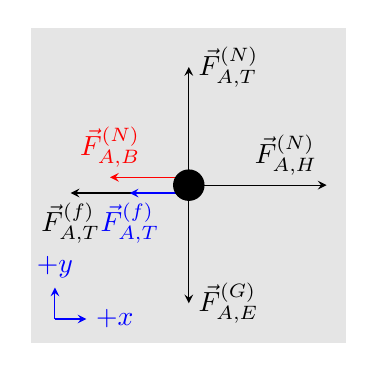
\begin{tikzpicture}
          \def\shift{0.1};
          \fill[black!10!white] (-2,-2) rectangle (2,2);
          \coordinate (O) at (0,0);
          \begin{scope}[->]
            \draw (O) -- +(0,-1.5) node [right]{$\vec{F}^{(G)}_{A,E}$};
            \draw (O) -- +(0,1.5) node [right]{$\vec{F}^{(N)}_{A,T}$};
            \draw (O) -- +(1.75,0) node [above left]{$\vec{F}^{(N)}_{A,H}$};
            \draw[red] ($(O) +(0,\shift)$) -- +(-1,0) node [above]{$\vec{F}^{(N)}_{A,B}$};
            \draw<1> ($(O) +(0,-\shift)$) -- +(-1.5,0) node [below]{$\vec{F}^{(f)}_{A,T}$};
            \draw<2->[blue] ($(O) +(0,-\shift)$) -- +(-0.75,0) node [below]{$\vec{F}^{(f)}_{A,T}$};
            \draw[blue] (-1.7,-1.7) -- +(0,0.4) node [above]{$+y$};
            \draw[blue] (-1.7,-1.7) -- +(0.4,0) node [right]{$+x$};
          \end{scope}
          \fill (O) circle (0.2);
        \end{tikzpicture}
      \end{center}
    \end{column}
    \begin{column}
      {0.45\textwidth}
      System B
      \begin{center}
        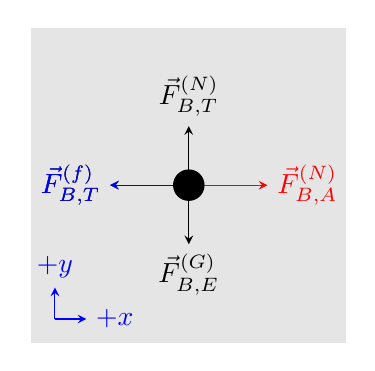
\begin{tikzpicture}
          \fill[black!10!white] (-2,-2) rectangle (2,2);
          \coordinate (O) at (0,0);
          \begin{scope}[->]
            \draw (O) -- +(0,-0.75) node [below]{$\vec{F}^{(G)}_{B,E}$};
            \draw (O) -- +(0,0.75) node [above]{$\vec{F}^{(N)}_{B,T}$};
            \draw<1> (O) -- +(-1,0) node [left]{$\vec{F}^{(f)}_{B,T}$};
            \draw<2->[blue] (O) -- +(-1,0) node [left]{$\vec{F}^{(f)}_{B,T}$};
            \draw[red] (O) -- +(1,0) node [right]{$\vec{F}^{(N)}_{B,A}$};
            \draw[blue] (-1.7,-1.7) -- +(0,0.4) node [above]{$+y$};
            \draw[blue] (-1.7,-1.7) -- +(0.4,0) node [right]{$+x$};
          \end{scope}
          \fill (O) circle (0.2);
        \end{tikzpicture}
      \end{center}
    \end{column}
  \end{columns}
  \uncover<2>{
    Only the \textcolor{blue}{frictional forces} should decrease
  }
\end{frame}

\begin{frame}{Part \textrm{III}. Dealing with systems}
  Same as Part \textrm{II}, acceleration is constant and \textit{to the right}
  
  System C
  \begin{center}
    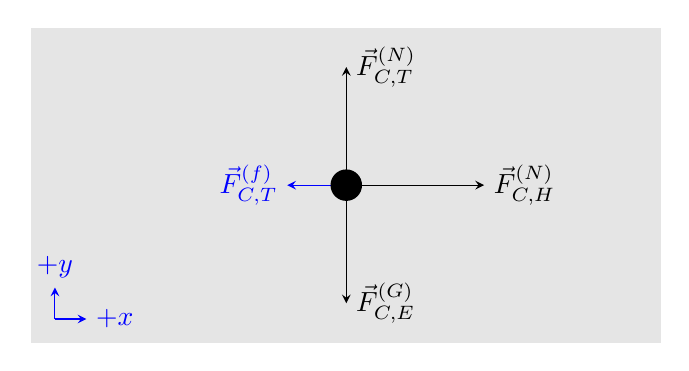
\begin{tikzpicture}
      \def\shift{0.1};
      \fill[black!10!white] (-4,-2) rectangle (4,2);
      \coordinate (O) at (0,0);
      \begin{scope}[->]
        \draw (O) -- +(0,-1.5) node [right]{$\vec{F}^{(G)}_{C,E}$};
        \draw (O) -- +(0,1.5) node [right]{$\vec{F}^{(N)}_{C,T}$};
        \draw (O) -- +(1.75,0) node [right]{$\vec{F}^{(N)}_{C,H}$};
        \draw<2->[blue] (O) -- +(-0.75,0) node [left]{$\vec{F}^{(f)}_{C,T}$};
        \draw[blue] (-3.7,-1.7) -- +(0,0.4) node [above]{$+y$};
        \draw[blue] (-3.7,-1.7) -- +(0.4,0) node [right]{$+x$};
      \end{scope}
      \fill (O) circle (0.2);
    \end{tikzpicture}
  \end{center}
  \begin{columns}[t]
    \begin{column}{0.4\textwidth}
      Corresponding forces:
      \begin{align*}
        \vec{F}^{(N)}_{C,T} &= \vec{F}^{(N)}_{A,T} + \vec{F}^{(N)}_{B,T} \\
        \vec{F}^{(f)}_{C,T} &= \vec{F}^{(f)}_{A,T} + \vec{F}^{(f)}_{B,T} \\
        \vec{F}^{(G)}_{C,E} &= \vec{F}^{(G)}_{A,E} + \vec{F}^{(G)}_{B,E} \\
      \end{align*}
    \end{column}
    \begin{column}{0.5\textwidth}
      Missing Forces: 
      \begin{itemize}
        \item $\vec{F}^{(N)}_{A,B}$
        \item $\vec{F}^{(N)}_{A,B}$
        \item These are \textit{internal} to the system
      \end{itemize}
    \end{column}
  \end{columns}
\end{frame}
\end{document}